\documentclass[tikz,border=5pt]{standalone}
% v3: data-led scientific illustration grammar. No dashboard cards or banners.
\usepackage{fix-cm}
\usepackage{amsmath,amssymb,graphicx}
\usepackage{tikz}
\usetikzlibrary{positioning,calc,fit,backgrounds,patterns,decorations.pathreplacing}
\renewcommand{\familydefault}{\sfdefault}
\definecolor{Ink}{HTML}{203848}
\definecolor{Muted}{HTML}{657884}
\definecolor{Rule}{HTML}{D2DDE3}
\definecolor{Observed}{HTML}{4E7897}
\definecolor{Teal}{HTML}{318E83}
\definecolor{Orange}{HTML}{C98542}
\definecolor{PaleBlue}{HTML}{EAF1F6}
\definecolor{PaleTeal}{HTML}{E8F3F0}
\definecolor{PaleOrange}{HTML}{FBF1E7}
\definecolor{GrayFill}{HTML}{F1F4F6}
\newcommand{\figfont}{\sffamily\fontsize{9.5}{11.5}\selectfont}
\newcommand{\figsmall}{\sffamily\fontsize{9}{10.5}\selectfont}
\tikzset{
 every node/.style={font=\figfont,text=Ink,inner sep=2pt},
 label/.style={font=\figfont,align=center},
 small/.style={font=\figsmall,text=Muted,align=center},
 panelletter/.style={font=\sffamily\bfseries\fontsize{10}{12}\selectfont,anchor=west},
 operator/.style={draw=Rule,fill=white,line width=.65pt,minimum height=.55cm,align=center,inner sep=4pt},
 flow/.style={->,>=stealth,draw=Ink!85,line width=.75pt},
 weight/.style={->,>=stealth,draw=Muted,dashed,line width=.65pt},
 axis/.style={->,>=stealth,draw=Muted,line width=.5pt},
 hair/.style={draw=Rule,line width=.5pt},
 sum/.style={circle,draw=Ink,fill=white,line width=.65pt,minimum size=12pt,inner sep=0pt},
}
% Illustrative 4x5 target table, not learned weights or experimental measurements.
% State 0: missing white; 1: initializer gray; 2: missing values restored in teal.
% Coordinates span [0,1.55] x [0,1.24]. No Other column is implied in this glyph.
\newcommand{\DataGrid}[1]{%
 \foreach \r in {0,...,3}{\foreach \c in {0,...,4}{%
  \pgfmathtruncatemacro{\tone}{25+mod(\r*17+\c*23,55)}
  \pgfmathtruncatemacro{\miss}{(\r==0&&\c==3)||(\r==1&&\c==0)||(\r==2&&\c==2)}
  \ifnum\miss=1
   \ifnum#1=0 \fill[white] (\c*.31,\r*.31) rectangle ++(.31,.31);
   \else\ifnum#1=1 \fill[Muted!22] (\c*.31,\r*.31) rectangle ++(.31,.31);
   \else \fill[Teal!65] (\c*.31,\r*.31) rectangle ++(.31,.31);\fi\fi
  \else \fill[Observed!\tone] (\c*.31,\r*.31) rectangle ++(.31,.31);\fi
  \draw[white,line width=.7pt] (\c*.31,\r*.31) rectangle ++(.31,.31);
 }}
 \draw[draw=Rule,line width=.55pt] (0,0) rectangle (1.55,1.24);
}
% A C-channel token is shown as a compact stack of editable vector strips.
\newcommand{\ChannelStrip}[1]{%
 \foreach \j in {0,...,7}{\pgfmathtruncatemacro{\tone}{25+mod(\j*17,55)}
  \fill[#1!\tone] (\j*.12,0) rectangle ++(.10,.43);}
}
\newcommand{\MaskGrid}{%
 \foreach \r in {0,...,3}{\foreach \c in {0,...,4}{%
  \pgfmathtruncatemacro{\miss}{(\r==0&&\c==3)||(\r==1&&\c==0)||(\r==2&&\c==2)}
  \ifnum\miss=1 \fill[white] (\c*.31,\r*.31) rectangle ++(.31,.31);
  \else \fill[Observed!55] (\c*.31,\r*.31) rectangle ++(.31,.31);\fi
  \draw[white,line width=.7pt] (\c*.31,\r*.31) rectangle ++(.31,.31);}}
 \draw[draw=Rule,line width=.55pt] (0,0) rectangle (1.55,1.24);
}
% Four parts x three real visits plus one padded row. Arrows identify axes,
% not numerical/learned attention weights. Mode 0 temporal; mode 1 feature.
\newcommand{\AxisGrid}[1]{%
 \fill[PaleBlue] (0,0) rectangle (1.28,1.28);
 \ifnum#1=0 \fill[Observed!22] (.32,.32) rectangle (.64,1.28);
 \else \fill[Teal!23] (0,.64) rectangle (1.28,.96);\fi
 \fill[GrayFill] (0,0) rectangle (1.28,.32);
 \foreach \i in {0,...,4}{
  \draw[draw=white,line width=.75pt] (\i*.32,0) -- (\i*.32,1.28);
  \draw[draw=white,line width=.75pt] (0,\i*.32) -- (1.28,\i*.32);}
 \draw[draw=Rule,line width=.5pt] (0,0) rectangle (1.28,1.28);
 \ifnum#1=0
  \draw[<->,>=stealth,draw=Observed,line width=1pt] (.48,.44) -- (.48,1.16);
 \else
  \draw[<->,>=stealth,draw=Teal,line width=1pt] (.12,.80) -- (1.16,.80);\fi
}

% Exact operator trace: network.py:40--60. One block, three local residuals.
\begin{document}
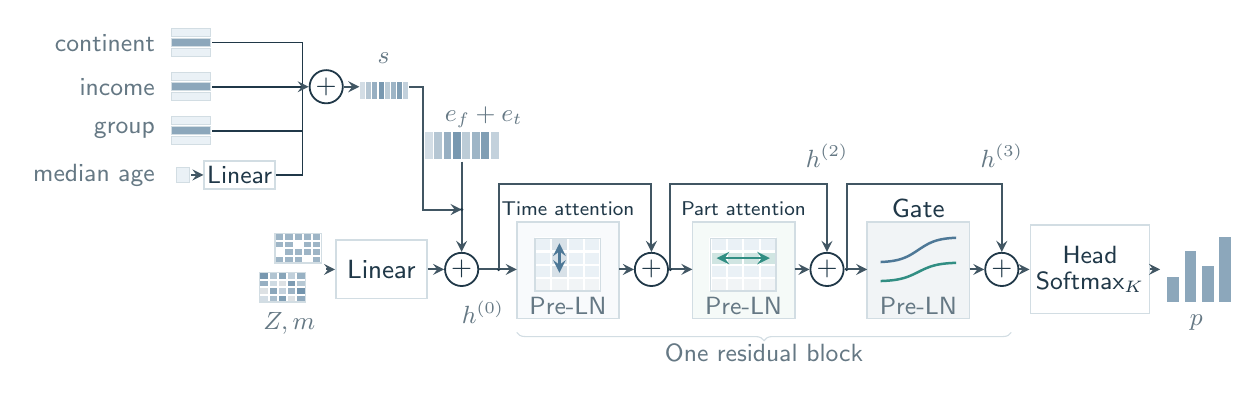
\begin{tikzpicture}[y=.8cm]
 \begin{scope}[shift={(0,.78)},scale=.38]\DataGrid{1}\end{scope}
 \begin{scope}[shift={(.20,1.40)},scale=.38]\MaskGrid\end{scope}
 \node[small] at (.38,.45) {$Z,m$};
 \node[operator,minimum width=.86cm,minimum height=.74cm] (lift) at (1.55,1.30) {Linear};
 \node[sum] (embedding) at (2.57,1.30) {$+$};
 \draw[flow] (.85,1.30) -- (lift);
 \draw[flow] (lift) -- (embedding);
 \begin{scope}[shift={(2.10,3.05)}]\ChannelStrip{Observed}\end{scope}
 \node[small] at (2.85,3.72) {$e_f+e_t$};
 \draw[flow] (2.57,3.01) -- (embedding.north);
 \node[small] at (2.84,.62) {$h^{(0)}$};


 % Four static fields form one shared vector.
 \foreach \y/\name in {4.9/continent,4.2/income,3.5/group}{
  \node[small,anchor=east] at (-1.25,\y) {\name};
  \foreach \r in {0,1,2} {
   \ifnum\r=1 \def\rowfill{Observed!65}\else\def\rowfill{PaleBlue}\fi
   \draw[draw=Rule,fill=\rowfill,line width=.35pt] (-1.12,\y-.22+\r*.16) rectangle ++(.50,.13);
  }
  \draw[draw=Ink,line width=.6pt] (-.60,\y) -- (.55,\y) -- (.55,4.2);
 }
 \node[small,anchor=east] at (-1.25,2.8) {median age};
 \draw[draw=Rule,fill=PaleBlue] (-1.05,2.68) rectangle ++(.16,.24);
 \node[operator,font=\figsmall,minimum width=.6cm,minimum height=.35cm,inner sep=1pt] (age) at (-.25,2.8) {Linear};
 \draw[flow] (-.87,2.8) -- (age);
 \draw[draw=Ink,line width=.6pt] (age.east) -- (.55,2.8) -- (.55,4.2);
 \node[sum] (msum) at (.85,4.2) {$+$};
 \draw[flow] (.55,4.2) -- (msum);
 \begin{scope}[shift={(1.28,4.00)},scale=.65]\ChannelStrip{Observed}\end{scope}
 \draw[flow] (msum.east) -- (1.27,4.2);
 \node[small] at (1.58,4.65) {$s$};
 \draw[flow] (1.90,4.2) -- (2.08,4.2) -- (2.08,2.25) -- (2.57,2.25);
 \fill[Ink] (2.57,2.25) circle (.65pt);
 % Visual operators carry the mechanism; detailed shapes belong to captions.
 \path[draw=Rule,fill=PaleBlue!35,line width=.6pt] (3.27,.52) rectangle (4.57,2.05);
 \begin{scope}[shift={(3.50,.96)},scale=.65]\AxisGrid{0}\end{scope}
 \node[label,font=\fontsize{7.2}{8.2}\selectfont] at (3.92,2.27) {Time attention};
 \node[small] at (3.92,.72) {Pre-LN};
 \coordinate (tin) at (3.27,1.30);\coordinate (tout) at (4.57,1.30);
 \node[sum] (tr) at (4.98,1.30) {$+$};
 \draw[flow] (embedding.east) -- (tin);
 \draw[flow] (tout) -- (tr);
 \fill[Ink] (3.04,1.30) circle (.65pt);
 \draw[flow] (3.04,1.30) -- (3.04,2.65) -- (4.98,2.65) -- (tr.north);

 \path[draw=Rule,fill=PaleTeal!45,line width=.6pt] (5.50,.52) rectangle (6.80,2.05);
 \begin{scope}[shift={(5.73,.96)},scale=.65]\AxisGrid{1}\end{scope}
 \node[label,font=\fontsize{7.2}{8.2}\selectfont] at (6.15,2.27) {Part attention};
 \node[small] at (6.15,.72) {Pre-LN};
 \node[sum] (fr) at (7.21,1.30) {$+$};
 \draw[flow] (tr) -- (5.50,1.30);
 \draw[flow] (6.80,1.30) -- (fr);
 \fill[Ink] (5.22,1.30) circle (.65pt);
  \draw[flow] (5.22,1.30) -- (5.22,2.65) -- (7.21,2.65) -- (fr.north);
  \node[small] at (7.21,3.10) {$h^{(2)}$};

 \path[draw=Rule,fill=GrayFill,line width=.6pt] (7.72,.52) rectangle (9.02,2.05);
 \node[label] at (8.37,2.27) {Gate};
 \draw[Observed,line width=.9pt,domain=-1:1,samples=31,smooth]
  plot ({8.37+.48*\x},{1.61+.20*tanh(2*\x)});
 \draw[Teal,line width=.9pt,domain=-1:1,samples=31,smooth]
  plot ({8.37+.48*\x},{1.11+.30/(1+exp(-4*\x))});
 \node[small] at (8.37,.72) {Pre-LN};
 \node[sum] (gr) at (9.43,1.30) {$+$};
 \draw[flow] (fr) -- (7.72,1.30);
 \draw[flow] (9.02,1.30) -- (gr);
 \fill[Ink] (7.46,1.30) circle (.65pt);
  \draw[flow] (7.46,1.30) -- (7.46,2.65) -- (9.43,2.65) -- (gr.north);
  \node[small] at (9.43,3.10) {$h^{(3)}$};

 \node[operator,font=\figsmall,minimum width=1.35cm,minimum height=1.12cm,inner sep=2pt]
  (head) at (10.55,1.30) {Head\\[-1pt]Softmax$_K$};
 \draw[flow] (gr) -- (head);
 \draw[flow] (head.east) -- (11.44,1.30);
 \foreach \x/\h in {11.53/.40,11.75/.82,11.97/.58,12.19/1.04}
  \fill[Observed!65] (\x,.78) rectangle ++(.15,\h);
 \node[small] at (11.90,.45) {$p$};
 \draw[draw=Rule,decorate,decoration={brace,mirror,amplitude=3pt}]
  (3.27,.30) -- (9.55,.30);
 \node[small] at (6.41,-.02) {One residual block};
\end{tikzpicture}
\end{document}
